\documentclass[12pt,twoside,a4paper,openright]{book}
%\usepackage[utf8]{inputenc}
\usepackage{floatflt,graphicx}           % Floating figures
\usepackage{euler}
\usepackage{float} %'H' for figures
\usepackage{array}
\usepackage{amsmath} %Math
\usepackage{texdraw} %Gnuplot
\usepackage[all]{xy} % Graphs with text
\usepackage{algorithmic}
\usepackage{xspace}
\usepackage{listings}
\usepackage{pdfpages}
\usepackage{subfigure}
\usepackage[parfill]{parskip}
%\usepackage{fullpage}
%\usepackage{titlesec}
\usepackage{listings}

\usepackage[printonlyused]{acronym}

%\setlength{\parindent}{0pt}
%\setlength{\parskip}{\baselineskip}
%\titlespacing\section{0pt}{12pt plus 4pt minus 2pt}{-6pt plus 2pt minus 2pt}

\begin{document}

\DeclareGraphicsExtensions{.pdf,.png,.jpg}

\renewcommand{\bibname}{References}
\renewcommand{\contentsname}{Table of Contents}

\newcommand{\TIL}{Troms{\o} IL\xspace}
\newcommand{\SIF}{Str{\o}msgodset \xspace}

% Referencing macros
\newcommand{\s}[1]{Section~\ref{#1}}
\newcommand{\f}[1]{Fig.~\ref{#1}}
\renewcommand{\t}[1]{Table~\ref{#1}}

% Defining macros
\newcommand{\Section}[1]{%
 \section {#1}
 \label {sec:#1}
 \acresetall%
}

\newcommand{\Subsection}[1]{%
 \subsection {#1}
 \label {sec:#1}%
}
% Image definition
\newcommand{\PdfImage}[2]{%
 \begin{figure}
  \centering
  \includegraphics[page=#1,width=\linewidth]{images}
  \caption{#2}
  \label{pdf:#1}
 \end{figure}
} 

\newcommand{\PngImage}[3]{%
 \begin{figure}[H]
  \centering
  \includegraphics[width=\linewidth]{#3}
  \caption{#1}
  \label{png:#2}
 \end{figure}
} 

\pagestyle{empty}

\sloppy

\includepdf[pages=1]{frontpage.pdf}
\cleardoublepage
\pagenumbering{roman}
\pagestyle{plain}

\chapter*{Abstract}
Sports science is an increasingly hot topic and more and more soccer teams are investing time and money into strategic development of big data and sports science. All this to increase the players performance on the field and reduce the risk of injuries. Soccer teams and athletes in general are constantly looking for possibilities to gain advantages over opponents. In soccer your next opponent is analyzed down to the smallest details to find weaknesses and strengths. All this to be able to take advantage of your opponents weak points and limits their strengths.

This project creates and evaluates a system for capturing events relevant for opponent analysis and an interface providing the information for analyzing soccer opponents.




\chapter*{Acknowledgements}


%%
%
%%% Table of content
\setcounter{secnumdepth}{3}
\setcounter{tocdepth}{3}
\tableofcontents	

\chapter{List of Acronyms}
\begin{acronym}

\acro{UI}{User Interface} % Example
\acro{GUI}{Graphically User Interface} % Example
\acro{TIL}{Troms{\o}  Idrettslag}
\acro{ZXY}{ZXY Sport Tracking System}
\acro{AJAX}{Asynchronous JavaScript and XML}
\acro{JSON}{JavaScript Object Notation}
\acro{HTML}{HyperText Markup Language}
\acro{CSS}{Cascaading Style Sheets}
\acro{API}{Application Programming Interface}
\acro{REST}{Representational state transfer}
\acro{HTTP}{Hypertext Transfer Protocol}
\acro{MVP}{Model View Presenter}
\acro{DOM}{Document Object Model}
\acro{XML}{eXtensible Markup Language}
\acro{SPA}{Single Page Application}

\end{acronym}


\listoffigures

\listoftables

\pagestyle{plain}
\cleardoublepage
\pagenumbering{arabic}
% Introduction
\chapter{Introduction} \label{Introduction}
\section{Background}

Sports science is an increasingly hot topic and more and more soccer teams are investing time and money into strategic development of big data and sports science \cite{bigdata:majorleague}. All this to increase the players performance on the field and reduce the risk of injuries. One of the pioneers in this field for a long time AC Milan established in as early as 2002 the MilanLab \cite{bigdata:milanlab}. The goal for the program was to get better and more concrete information about the player’s physicality by collecting data over time of player’s performance. As AC Milan was one of the first to use big data, the use of big data today has exploded. Services like Opta and Prozone serves player statistics, heat maps, and video analytics of player’s performance. Fans get exposed to these statistics by clubs and broadcasting companies that uses it actively in their coverage of soccer games. The awareness of statistics for clubs and fans has possible never been higher than now \cite{dailymailOnStatistics}.

Soccer teams and athletes in general are constantly looking for possibilities to gain advantages over opponents. In soccer your next opponent is analyzed down to the smallest details to find weaknesses and strengths. All this to be able to take advantage of your opponents weak points and limits their strengths. The players should know what to expect from the opponent team. Detecting typical team plays and player movement of your opponent can help you prepare for the match. 

There are several ways to gather information about your opponent; from looking through whole matches to advanced tools, which can highlight key information for you. Some of them are expensive as Prozone \cite{Prozone:indepth} which is a complete system for capturing and presenting information. For small soccer clubs with relatively small budgets this can be a expensive investment. Another system is Interplay Sports, which Tromsø IL uses for game analytic. A video feed from any match can be used as the input letting you manually tag and describe situations in the match. In a sport where the next soccer match usually is in 3 days tools for filtering out the useless data is valuable.

In the analytic process there are two processes we will look at; first you need to gather the information and secondly is how to present the information gathered. 

\section{Problem definition}

This project will develop a system complementing the Muithu and Bagadus systems. Focus will be on soccer opponent analytics, where a data repository needs to be developed capturing important events relevant for this type of analytics. Especially we want to identify the key players offensive in a team. A user interface component providing the core information about the opponent should also be developed.

\section{Interpretation}

The project is that providing an infrastructure for capturing events like attacks that leads to an attempt on the opponent goal, and presenting this information through a user interface. We are interested in how long it typically takes to capture all relevant events from a single match, as this has to be done manually. A data model that reflects what we want to capture from each attack needs to be developed for being able to get relevant information for being used as a opponent analytic system.

First a requirement specification shall be developed. Then a prototype and that fulfills the requirements. At last specialist in the domain of soccer shall evaluate the system.

The design and development processes will be performed in collaboration with staff of the Norwegian soccer club Trømsø IL. An end-user comparison of the system against currently available tools will perform a final evaluation, and the result of this evaluation will be used to conclude the project.

\section{Methodology}

The final report of the ACM Task Force on the Core of Computer Science \cite{computing_as_a_discipline} divides the discipline of computing into three major paradigms:

\begin{itemize}
\item \emph{Theory}: 
Theory: Rooted in mathematics, the approach is to define problems, propose theorems and look to prove them in order to find new relationships and progress in computing.
\item \emph{Abstraction}: 
Rooted in the experimental scientific method, the approach is to analyze a phenomenon by creating hypothesis, constructing models and simulations, and analyzing the results.
\item \emph{Design}: 
Rooted in engineering, the approach is to state requirements and specifications, design and implement systems that solve the problem, and test the systems to systematically find the best solution to the given problem.

\end{itemize}

For this project the design process seems to be the most suitable out of the three paradigms. The design process consists of 4 steps, which are repeated if tests reveal that the latest version of the system does not meet the requirements.

\begin{itemize}
\item \emph{State requirements and specification}: A need or problem is identified, researched, and defined.
\item \emph{Design and implement the system}: Data models and a system architecture are designed. Prototypes are implemented.
\item \emph{Test the system}: Assessment and testing of the aforementioned prototypes.
\end{itemize}

\section{Outline}

\begin{itemize}
\item \emph{Chapter 2}: Presents some related work to the project
\item \emph{Chapter 3}: Describes the requirement specification
\item \emph{Chapter 4}: Describes the design and implementation of the system
\item \emph{Chapter 5}: Gives a demonstration of the system
\item \emph{Chapter 6}: Evaluates and discuss the system
\item \emph{Chapter 7}: Concludes the project 
\end{itemize}




\acresetall
% Background
\chapter{Related work} \label{Background}


In this chapter we present some background related to analytic in the domain of soccer . We look at types of analysis out there. This spans from pre-match to post-match. Then we go into how data is gathered and presented. There are two main approaches for capturing data: manually often by human annotating it, and automatic capturing often by using sensors.

\section{Types of analysis}

In soccer there are several phases where you use analytic to help you gain insight. Not only the soccer team uses analytics, but TV and fans also.

\subsection{Prematch}

Pre-match you use analytic to find weaknesses and strengths in the opponent team, on a individually level or as a team. You look at your team matched up against your opponent. A typical situation is that the manager gets an video summary of the opponent highlighting the opponents strengths and weaknesses. The video summary is often made up by the coaching staff who may use tools like Interplay. 

Typically in TV you have pundits bringing you analytic of key battles during the build up to the game. 

\subsubsection{In match}

During match the coaching staff continuously analysis the match and makes adjustment. Of course it is the players who makes all the decisions in the end, but the coach is the boss and most of the time players listen to what hes says. An adjustment to the formation can potentially be the tipping point in the game.

Tromsø IL uses a system Muithu that lets you annotate sequences of a game with entity's like player, comment. This information will then be time synchronized with the video feed. Later, like in the break or in the game even, you can search on entity's to get the corresponding video feed. As the system is available on an tablets players can in the middle of the match come to sideline to see a involvement. It can be anything that is tagged like a player involvement to a team move.

Using systems like ZXY or MiCoach you can get real time information about a players performance. Rather than guessing that a player is tiering during a game you can get information metrics. You get an evidence based on the metrics you get that the player in fact looks fatigued. In soccer you only have 3 substitutions. Making the right ones is crucial.

Using data gathered from sports data company like Opta you can get statistics live during the game. Its popular in TV to show statistics like ball possession percent, how far players have run or passes played and so on. 

\subsubsection{Post match}

During the post match the coach team goes through the game to evaluate the team performance. This is valuable as you get very concrete information about good and bad. You can highlight situations in the match to help players understand tactical aspects.

\section{Manually capturing }

\subsection{Opta }


One of the big players Opta uses manual input to create their data repository. They have editorial teams across the world that captures data manually for the most popular soccer leagues and other sports. For example to capture statistics for one match, 3 humans have to be involved to be able to annotate all data. The data is captured via an application specifically created for the purpose of capturing data as quick and easily as possible. The editorial teams of Opta need to be able to identify a player, registrate a pass his made or a tackle, in a very short time to be able to keep up with the pace of the game. They study things like which shoe color a player has to be able to quickly identify a player.

Opta capture all types of actions like passes, type of pass, attacks, and interceptions. For each action they log they add a series of description tags like pitch coordinate, player, team and time-stamp. For every single pass they registrate if it was a through ball, normal ball or even a headed flick on from a long ball. For shots they registrate the foot it was kicked with, if it was a volley and so on . All this is done while the match is playing. About 1600 individual events are recorded in a standard match. 

\begin{lstlisting}
<Event id="290575408" event_id="5" type_id="1" period_id="1" 
min="0" sec="5" player_id="20856" team_id="810" outcome="1" 
x="44.6"y="61.1" timestamp="2007-08-12T13:00:24.827" 
last_modified="2007-08-12T13:00:25">
<Q id="1774596260" qualifier_id="141" value="91.6"/>
<Q id="1429253465" qualifier_id="140" value="49.9"/>
<Q id="1084400575" qualifier_id="56" value="Back"/>
</Event>
\end{lstlisting}

Above is an example of an event registrated in the Opta database. The event has a series of qualifiers describing it. Except from the obvious as timestamp and last modified dates we see that the player id, team id, time of event, x and y coordinates and the outcome of the event are registrated. Also we see that some extra details are included. In this example it maps to a pass from [44.6, 61.1] to [91.6, 49.9]. 

\begin{lstlisting}
<Q id="1774596260" qualifier_id="coordX" value="91.6"/>
<Q id="1429253465" qualifier_id="coordY" value="49.9"/>
<Q id="1084400575" qualifier_id="56" value="Back"/>
\end{lstlisting}

\subsubsection{Prozone}
Prozone is a video-based system that tries to track players in team sports. Their data capture system incorporates 8-12 cameras, which is strategically positioned throughout the stadium to cover 100 percent of the ground, but with some redundancy in case of a faulty component. They also incorporate the TV-camera feed, which always follows the ball. All cameras are hooked into one server and uploaded at the end of the game before sent to undertake the tracking process. As different football grounds houses different pitch sizes the pitch dimensions has to be taken into account by calibrating the cameras. This is done when the system is installed by an operator. 

\begin{figure}[ht!]
\centering
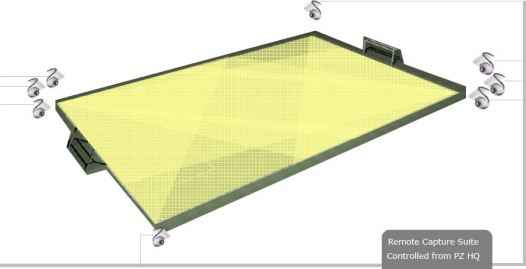
\includegraphics[width=150mm]{images/general/prozonecam.png}
\caption{The Prozone camera system illustrated}
\label{overflow}
\end{figure}

The coding and tracking process of the players movement and actions is a sort of manual process at present time. First each camera feed goes through each own tracking process determining image co-ordinates and continuous trajectories for each player.The output from all the cameras is then combined into one dataset. Going into the algorithm for this is out of the scope of this project. In the final stage the manual work comes into the loop. There has to be a quality control group of operators dedicated for post processing the game. First the operators has to map the players identity and with the their corresponding start location. The operators will then follow the video feed checking that the identification of all players remain constant during the match. The tracking process may run into problems when two players collide or have any other physical contact as it becomes unclear who is who. To map video image co-ordinates to pitch co-ordinates Prozone uses computer vision homography calibration process.

The whole input process is done in a own software which helps you minimize the amount of manual work for the operators. The software follows rules created by basic machine learning algorithms to validate and verify the input. A simple example would be if the ball goes out of play the system will now that the next event will be a throw in, corner kick or goal kick \cite{Prozone:indepth}.

Prozone claims to be able to track every movements of every player on the pitch every 10th of a second without using any physical equipment on the players. Di Salvo et al. \cite{Prozone:validation} conducted an empirical evaluation of deployed ProZone systems at Old Trafford in Manchester and Reebook Stadium in Bolton, and concluded that the video camera deployment gives an accurate and valid motion analysis. The data is after a match available through the PROZONE3 interface for analysis. 

\subsection{Automatic capturing}

A system that uses sensors is the ZXY sport trackingsystem \cite{ZXY:mainsite}. The system is in used by premier league soccer teams in Norway, including Tromsø IL and Rosenborg BK. Data captured is stored in Sybase databases with each match requiring about 500-700MB storage  The players have to wear a belt around their waist for the system to be able to track their movements. The ZXY system is able to track the players movement very detailed with an accuracy of 0.5m. It has a resolution of 20 samples per second. The technology behind it relies on a radio-based signaling substrate to provide real-time high-precision positional tracking, also including acceleration and heart rate. A installation of receivers is required for the system to work. The home arena for Tromsø IL, Alfheim, is currently equipped with 10 receivers . A receiver tracks an specific area of the soccer field and combined they cover the whole pitch with some redundancy areas. The communication from the belt to the receivers goes on a 2.45-5.2 G Hz frequency radio signal. To compute the positional data the stationary radio receiver uses an advance vector based processing of the received radio signal. The data is aggregated and stored into a relational database. Including the positions of the players the ZXY also gives you the step frequency and speed. 

\begin{figure}[ht!]
\centering
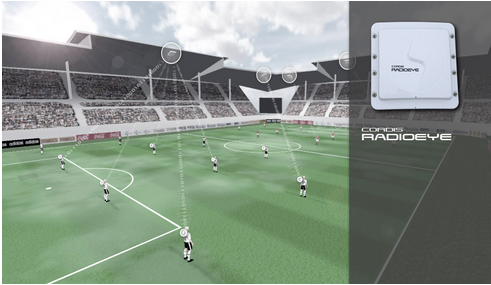
\includegraphics[width=150mm]{images/general/zxyoverview.png}
\caption{Overview of the ZXY system with receivers placed at the stadium and players wearing sensors}
\label{overflow}
\end{figure}


\subsection{Wrap up}
The main problem with tracking systems that uses physical sensors is that usually only one of the teams wears the sensors.  This limits the functionality of the system as a opponent analysis system. You only get data for one team. 

On the other hand you have the manually systems that requires some human annotation. These system are able to track both teams. As they rely on human annotation of some degree they get more rich data as well, but requires strict rules to not mess up the semantics. 


\subsection{Presenting data}

Most presenting of data is based around single matches. Figure 2.2 shows an example of how FourFourTwo presents data from a match. They use statistics from Opta. 

\subsubsection{Prozone}


Prozone comes with several softwares to illustrate the data. The most relevant for this project is the opposition analysis system. 

2D animation
Single player analysis
Team analysis
Pressing analysis
Success/direction
Player tempo
Passing movements
Receving the ball
Player events

\begin{figure}[ht!]
\centering
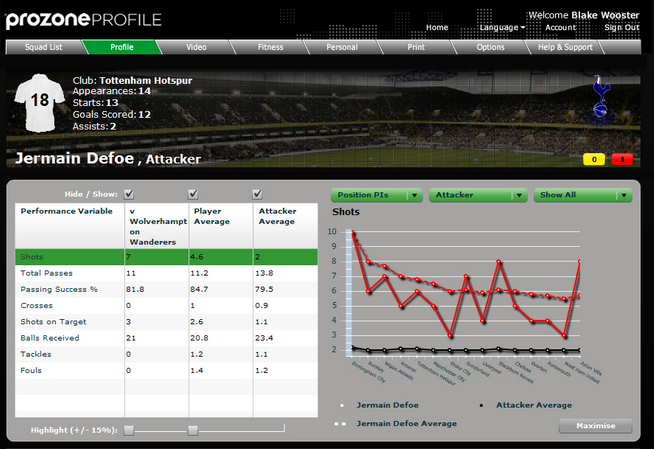
\includegraphics[width=100mm]{images/general/prozonestats.png}
\caption{The Prozone software - individual player analysis gives you statistics of performance over time}
\label{overflow}
\end{figure}

On individual level you can get basic tactics like shots, total passes, passing success, crosses, shots on target, balls received, tackles, fouls. 

Doing queries on the data can give you all sprints for a certain player. Players in certain areas of the field have more intensive sprints when they first are involved thus are more vulnerable to injuries. Knowing the actual physical load on players can prevent injuries by regulating the training intensity and amount of time on each exercise.

\subsubsection{ZXY}
  
ZXY provides you with a 3D graphic interface. This interface lets you see the players action in real time by reading the data stream to reproduce the players action. The data is streamed in real time into the database as the match goes on. While watching you can produce timestamps of different events and produce manual input which is time synchronized with the automatic data. Naturally you can build your own software on top of the Sybase database. Tromsø IL in collaboration with University of Tromsø has made several systems to complement the ZXY software. Muithu and Bagadus.

\begin{figure}[ht!]
\centering
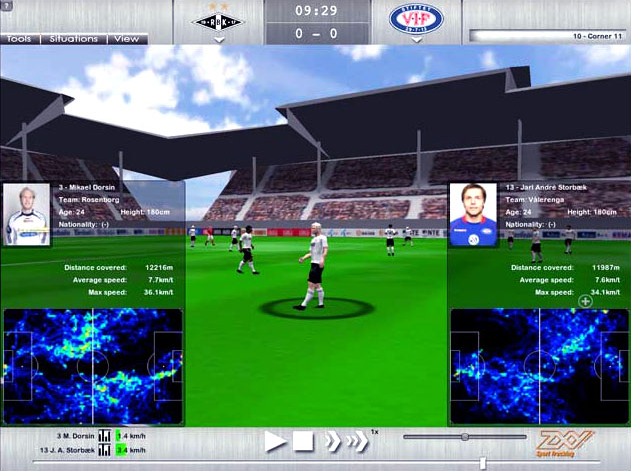
\includegraphics[width=100mm]{images/general/zxysoftware.png}
\caption{The ZXY software - tracking of players gives you information of distance covered, average speed and max speed. You also get a heat map of the players movement on the field.}
\label{overflow}
\end{figure}

\cite{dailymailOnStatistics}

\acresetall
% Requirements
\chapter{Requirement Specification} \label{Requirements}
This chapter outlines the requirement specification of the system. This section describes the requirement analysis process. The process of gathering the requirements was done in collaboration with Tromsø IL.

\section{Overview}

The requirements evolved during the process of developing the system. Initially a requirement specification was designed from our perspective. We looked at the different analyze systems out there and as mentioned in chapter 3 a good system for locating key players in opponent teams was lacking. Rather than going very wide providing all kind of analyses we narrowed it down to a very concrete system. A system that tries to to for many things may fell between two chairs, and at the end of the day not providing anything. You spend less time on each feature as you have more features thus reducing the quality on each feature.

The imagined system shall give you the key players in the offensive play of a given opponent soccer team. You shall be able to search on teams and individual players. Additionally you shall be able to see which areas of the pitch players are creating goal chances from. The system also needs a way of capturing data. This shall be an interface that enables you to store successful attacks for any match.

\begin{figure}[ht!]
\centering
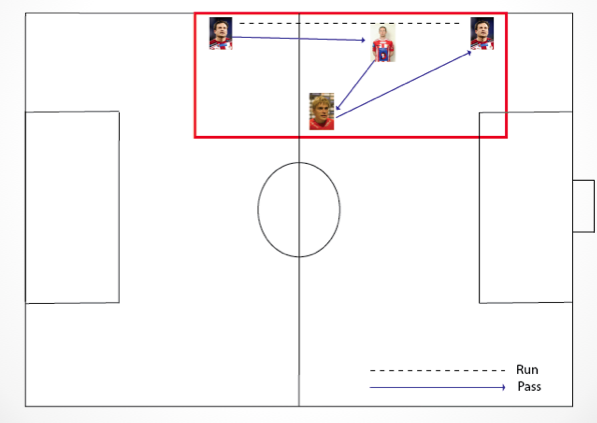
\includegraphics[width=50mm]{images/general/illustration_after_search.png}
\caption{Visioned illustration displaying key players and how they combine given you have queried on a team}
\label{overflow}
\end{figure}

\begin{figure}[ht!]
\centering
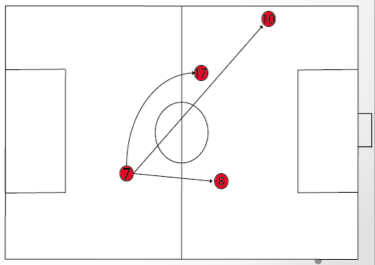
\includegraphics[width=50mm]{images/general/illustration_after_search2.png}
\caption{Visioned illustration of typical passes for a player}
\label{overflow}
\end{figure}

\section{Capture}

A domain model for the captured data is crucial to set early and don't change it radically. Initially we wanted to build a database of all the matches in the Norwegian premier league. From each match every successful attack a team makes should be captured. From the attack started you registrate where the attack started, every pass with from position to the new position, and type of attack. At last if there is a breaking point in the attack this should be captured. The breaking point of the attack is stored with a breakthrough player and what type of breakthrough it was.

Definition of breakthrough player: A player that does something extra that unbalance the other team. This can be a dribble past 1-2 players or a genius pass that opens deference of the opponents team. 

First problem was how to divide the pitch into zones. As we are looking for which zones the breaking point of the attack this is crucial for the searches on the data captured later on. During the development of the system several types of dividing was presented to the coaching staff. 

\begin{figure}[ht!]
\centering
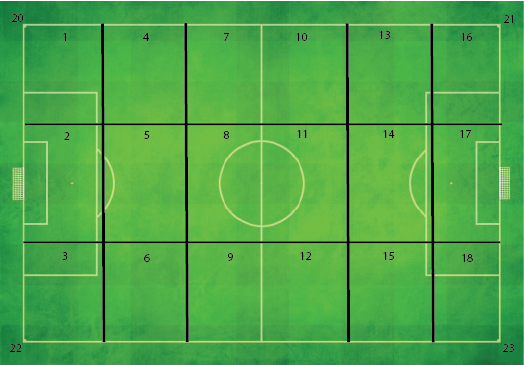
\includegraphics[width=100mm]{images/general/first_zones.png}
\caption{Dividing of pitch - the first suggestion had 18 zones. The team attacking attacks from left to right}
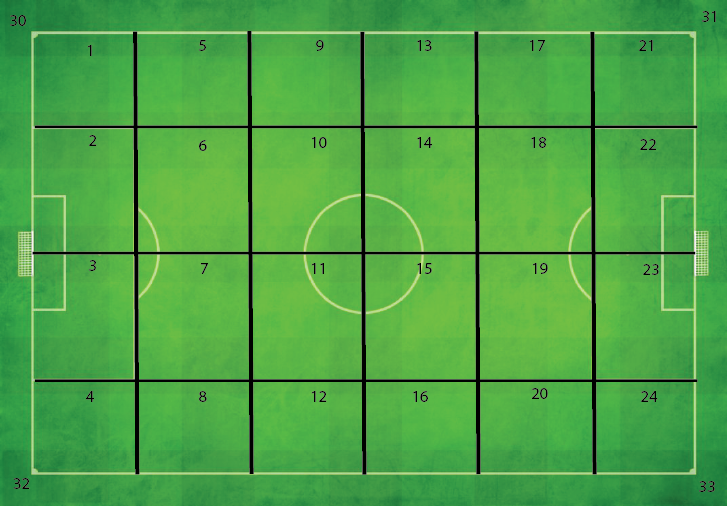
\includegraphics[width=100mm]{images/general/second_zones.png}
\caption{Dividing of pitch - the second suggestion had 18 zones. The team attacking attacks from left to right}
\label{overflow}
\end{figure}

\section{Present}
\acresetall

% Design
\chapter{Soccer Analytic toolkit (SAT)} \label{Design}


\section{System Architecture}

\begin{figure}[ht!]
\centering
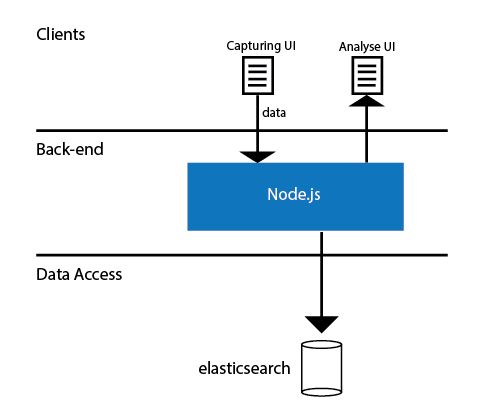
\includegraphics[width=100mm]{images/general/arhitecture.png}
\caption{Overall architecture of the system }
\label{overflow}
\end{figure}

The system architecture can be layered in to three layers; client, back-end, database. The control flow flows from the clients requesting something or inserting data, to the back-end and to the third layer, the database, and back up again in reverse order. 

\subsubsection{Interface}

The Soccer Analytic tool has one user interface - the web browser interface. Both the input and the analytic interface can be reached from this single web browser interface.

\subsubsection{Back-end}

The back-end is the middle layer between the client and the storage. Its main task is to serve static files to the clients, handle data insertions or handling web request by mapping them to database operations. New data insertions will possible be inserted into several database indexes. The back-end will then ensure that all indexes are updated before returning success to the client.

\subsubsection{Storage}

The storage layers task is to persist data and handle search queries on the data. It consist of several indexes that each store a part of domain the model. 

\subsection{Domain model}

The domain model is based around matches. All attacks is wrapped into a match root. Attacks can be seen as subdocuments of the match document. Inside the attacks all passes lies with other information. This gives a easy way of understanding how all the data is related together. Below is a complete example of how it all is structured. The number of attacks and passes is stripped down to one in the example.

\lstinputlisting{domainmodel.js}

\section{Implementation details}

\begin{figure}[ht!]
\centering
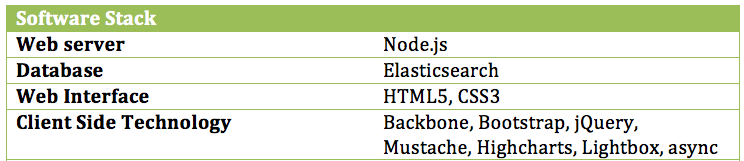
\includegraphics[width=100mm]{images/implementation/software_stack.png}
\caption{Software stack}
\label{overflow}
\end{figure}

\subsection{Storage}

The data storage is an elasticsearch database\footnote{http://www.elasticsearch.org/}. Elasticsearch is document oriented, schema less and works well with JSON\footnotemark. As our server is built on JavaScript working with JSON is easy. JSON-objects can be inserted right into the storage and elasticsearch will map fields and value accordingly, and make it available for search.
Elasticsearch takes advantages of embedded documents meaning we can store related data together. An attack is usually made up of several passes these can be stored as an embedded document in the attack document. Then all pases can be retrieved in one query when fetching an attack.

The main reason for using Elasticsearch is its search capability. In the starting phase of the project MongoDB \footnotemark was the storage engine. However as some aggregation queries was hard to figure out how to do a change to elasticsearch was made. It should be noted that MongoDB supports map reduce operations. With some extra work the queries causing problems could possible have been done with MongoDB. However, with elasticsearch you can in a single, simple to write query get counted how many passes all players for a team has played and received, the number of times all players has been the breakthrough-player in an attack, count type of attacks, count the most used zones for passing and finishing and so on. This makes it very easy and efficient to do queries for analyses on teams and players.

\footnotetext{http://www.json.org/}
\footnotetext{http://www.mongodb.org/}

\subsubsection{Indexes}

Indexes in much like tables in a relational database in the way that they is a container for data. An index stores documents which is a bunch of key/value pairs like JSON. You can let elasticsearch automatic analyze the field data or you can use mappings. For supporting querying on players and other fields where the value is more than one word, you have to tell elasticsearch that it is a multi field. For example searching for player name ''Stefan Johansen'' when the field is not set as multi field will give you two results and not one as you would expect.

In our project we have 5 different indexes. Team index which stores all the teams. Player index which stores all the players. Match index stores all data from a match including all attacks. Attack index stores information about attacks and last the pass index which stores passes. As may be noted there is data redundancy. You can argue that storage has become so cheap and if you can use a little bit extra space to gain performance you would do it. In this case it was done to be able to fully support aggregation functions on subdocuments.

\subsection{Back-end}

The back end is the middle-ware between the clients and the data layer. It exposes a RESTful\footnote{http://www.ibm.com/developerworks/webservices/library/ws-restful/} interface over HTTP for the client to communicate. A request coming in is transformed to a database query based on the resource it tries to access. On answer from the database the result is transformed before returning it to the client. 

Similar if the client sends new data for a match the middle-ware inserts the data into the appropriate indexes. The server will respond will HTTP status code 201 if all goes well or 400 on an error. The server uses HTTP code actively to tell the client the result of requests.

In principal, since the data input is generated in the web browser (with JavaScript), it could have been inserted right away into the database without going through an extra middleware. However, this limits us as we cant combine multiple queries by going through the back-end. Cleaning of data before serving to the client would neither be possible. Normally you also do validation of the data at the back-end before inserting into your database.

\subsubsection{API}

The API of the web server is listed in figure \ref{fig:api}.
\begin{figure}[ht!]
\centering
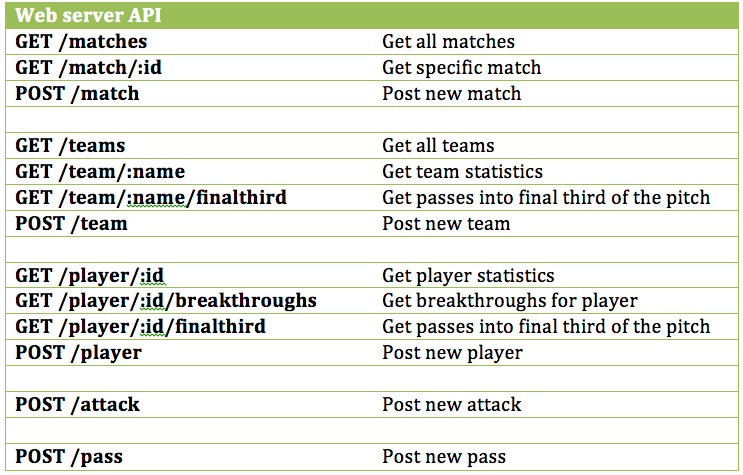
\includegraphics[width=100mm]{images/implementation/API.png}
\caption{Overview of the web servers API}
\label{fig:api}
\end{figure}

\subsection{Front-end}

Front end is consist of a single page JavaScript application using Backbone.js \footnotemark as under-supporting framework. Backbone uses a MVC model to structure the code. With Backbone your views will update automatic when data changes. In the following sections the architecture of the client and how different concepts is used will be described. 

\footnotetext{http://backbonejs.org/}

\begin{figure}[ht!]
\centering
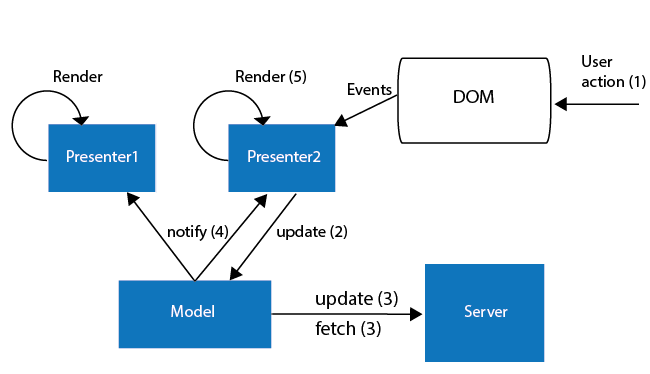
\includegraphics[width=150mm]{images/architecture/backbone_architecture.png}
\caption{Architecture of the client side}
\label{overflow}
\end{figure}

\subsubsection{Models}

Data is represented as models in backbone. The model has mainly two responsibilities. First is whenever a update on a models data occurs the model notifies the views that has subscribed for update events for that particular model. The second is that models is responsible for AJAX communication  with the back-end. An example is when a user registrates a new attack for a match. He fills out a form and press submit. Then a new Attack Model is created. Calling save on the instance of the model will send an AJAX post request to the server with the models data in the HTTP body.

Similar to a Attack Model we have Player Model that handles everything around players. When you click yourself into a players profile the model will fetch statistics from the back-end, notify the view that the data is ready, and the view will be rendered.

There is also a Match Model (fetching and registrating matches), Team Model (viewing statistics), and a Pass Model (saving passes). They work it the same way as the models described above.


\subsubsection{Views}

For a analytic toolkit to be useful a good UI is critical. Here several helper library is used to present the data. Highcharts.js\footnotemark  is a JavaScript library for illustrating graphs. A query on team generates a lot of statistics and rather than listing them up they are presented using charts. This also gives us the advantage of displaying several numbers for each player and plot it in the same graph. In figure \ref{fig:chart} the number of times a player has been involved in all attacks, number of passes into the final third of the pitch and the number of times a player has been the breakthrough-player is shown.

\footnotetext{http://www.highcharts.com/}

\begin{figure}[ht!]
\centering
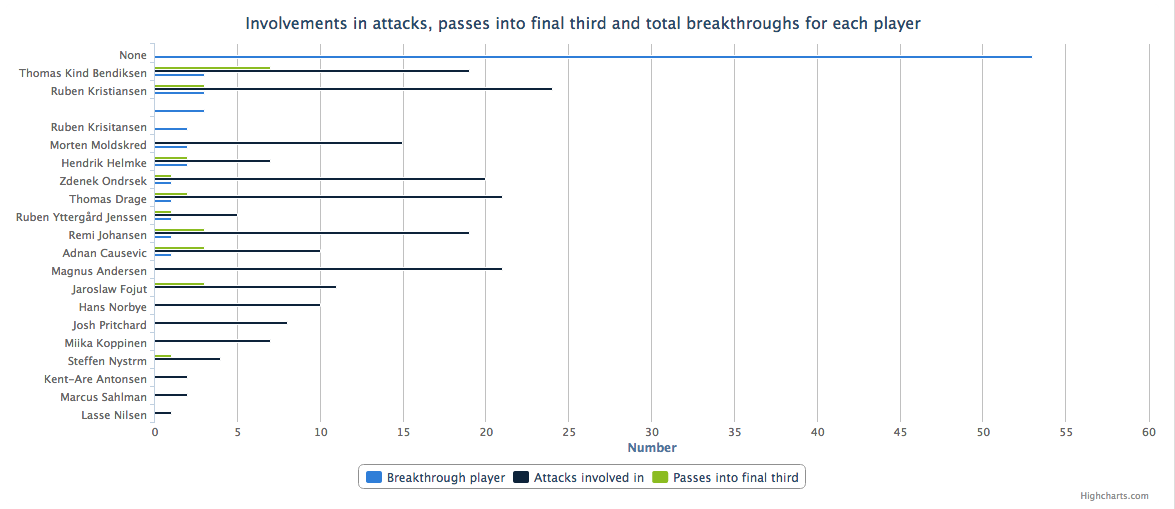
\includegraphics[width=100mm]{images/general/chart_passes.png}
\caption{Shows how the passing statistic is illustrated on the client by using Highcharts.js}
\label{fig:chart}
\end{figure}

Positional data is created using the a new feature of HTML5, canvas element. It lets you draw graphics on the fly in the web page. In this system it is used to create a element that symbols the different zones in our domain model. In the Team Model you have all zones with a number that symbols shots taken from that zone. This is then plotted into the respective zones.

\begin{figure}[ht!]
\centering
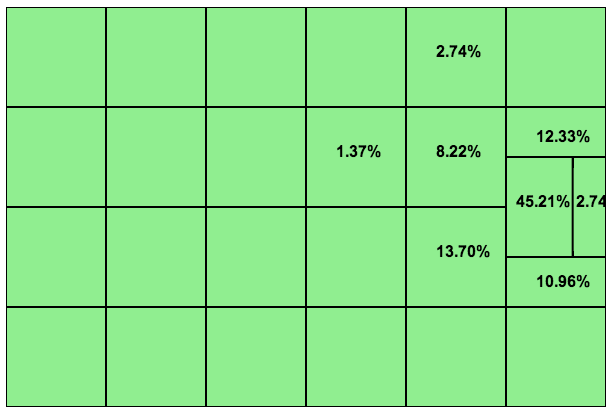
\includegraphics[width=85mm]{images/general/finishing_zones.png}
\caption{Illustrations of which zones the team has finished off their attacks from, with percent (team: Tromsø IL)}
\label{overflow}
\end{figure}

Backbone comes with a library Underscore.js\footnotemark that makes creating HTML pages with dynamic content easily. When you are rendering new content on the site you can insert data retried from a model dynamically into the HTML. In the example below the input is a an array of objects where each element in the array contains a key value pair 'name' : value. The html output of this will be a list of names.

\lstinputlisting{underscore_example.html}

\footnotetext{http://underscorejs.org/}

\subsubsection{Router}

A component not mentioned before that lies on the client is the router. The router is the glue that binds all the other moduels together. It handles the navigation between pages in the application. When users navigate on the page by clicking on links or buttons in a traditonal web page the back-end serves a new html page. In this page this click event is handled by a router module. The router model examins the URL request and routes the request to the mapped up view. The view is then responsible for calling fetch functions on the model and render the HTML.

ADD A SECOND ILLUSTRATION ADDNING THE ROUTER.

\subsection{Getting players and teams into the database}

Getting squads in a useful format like XML or JSON was harder than expected. On the norwegian football alliance's website you could download the squads for the current season only in PDF. Current squads is fetched from altomfotball.no, a website by the norwegian TV channel TV2. This is own python script meant to run only once to set up the database. For each team the script basically reads the HTML document with all players listed, parse out players name, and sends in to the web server.

MORE ON DEVELOPMENT PROCESS? How zone map changed etc. A change from Mongodb to elasticsearch


\subsection{Security}
Secturity is not taken into concern. This means anyone getting into the page can post new match data and add attacks. This could have been fixed by requiring a login before getting access to the site. 


\acresetall

% Demostration
\chapter{Demo} \label{Model}

\section{Interfaces}

The first page you are prompted with is the listing of all matches registered in the database. A click on match gives you details about that match and prompts you a interface for capturing new attacks if requested. Every field has to be submitted with an correct input value.

\begin{figure}[ht!]
\centering
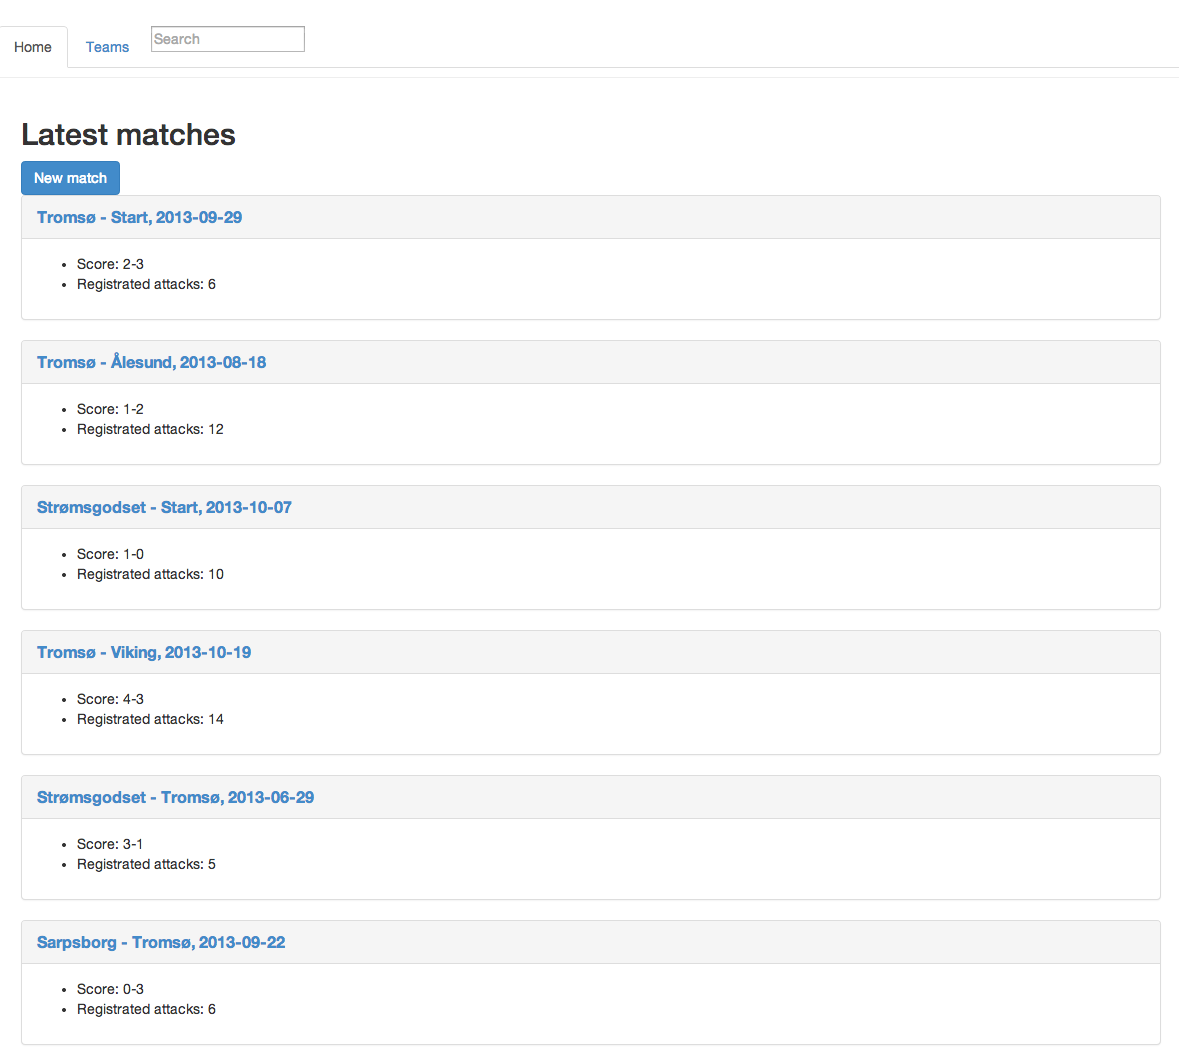
\includegraphics[width=100mm]{images/general/all_matches.png}
\caption{All matches registrated in the database are listed on this page}
\label{overflow}
\end{figure}

\acresetall

% Evaluation
\chapter{Evaluation and Results} \label{Evaluation}
This chapter presents methods used to evaluate the system; results collected evaluating the system and a discussion around the system. 

\section{Methods}
\subsection{User Survey}

The system is measured by doing user surveys on the end users. In our user survey we have coaches’ and others with many years of experience in soccer rating how much they agree with a statement on a Likert-scale. The statements compare the system against other systems in use at Alfheim today. For other’s we evaluate the system as a stand alone analytic system. The Likert-scale chosen is a 5 point scale from \textit{strongly disagree} to \textit{strongly agree}.\footnote{http://www.simplypsychology.org/likert-scale.html}. In short it will let each individual to note how much they disagree or agree with a particular statement.

We will also let assessors comment about the usability or other things of the system that will be taken into the evaluation. 

\subsection{UI Performance}

Measuring \ac{UI} Performance is way of measuring usability of the system. These two are directly linked up to each other \cite{satisfaction}. A slow system and unresponsive system decrease satisfaction and usability for the end-user. Foundings in \cite{nielsen} indicated that a response time of longer than 1000ms would decrease the satisfaction of the user. The thought-flow of the user will not be interrupted and therefor one can argue that the \ac{UI} it's fast enough. We will use this threshold to evaluate our UI performance in the system. 

To measure the UI Performance we use Google Chrome DevTools\footnote{https://developers.google.com/chrome-developer-tools/}. A web page is only fully loaded when all requests have been fully received. In our \ac{SPA} new requests will be spawned after the \ac{DOM} is loaded. Therefor, we run performance tests for both fully reload of the page, when the DOM is ready and when the users navigates in already rendered page, which will be the most typical way for the user to navigate to different pages.

\subsection{Compatibility}

In the requirement specification we stated that going for a web page would ensure compatibility and accessibility. Every device now has a web browser and therefor the page can be reached from anywhere as long as you have an Internet connection. 

To test this we use PowerMapper\footnote{ http://try.powermapper.com/demo/sortsite } website testing and site mapping tool. This test checks a wide range of things like browser support, dead links and accessibility. We use it to for compatibility testing for web browsers.

\section{Experiments and Results}

In the tests \ac{TIL} have been used to evaluate the system. In the tests we are looking to see if we have achieved or goals listed in the requirements. To recapture the main goals; we wanted to identify key players in soccer opponent teams and we wanted to create a system that difference it from the existing systems and at the same time provides valuable information for opponent soccer analytic. 

\subsection{Database size}
In figure \ref{fig:dbsize} the size of the different indexes in the database is listed. Match related data is stored in the match, attack and pass index. The total size of those 3 indexes is 379.5kb and with a total of 12 matches in the database. This means that an average match stored takes around 31.6kb of storage.

\begin{figure}[ht!]
\centering
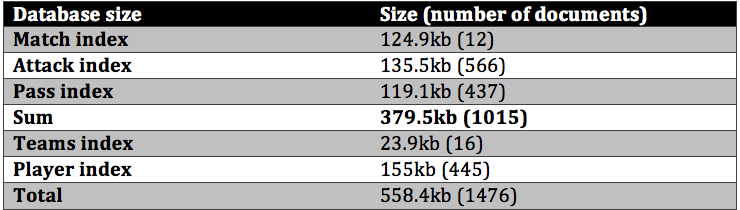
\includegraphics[width=1\textwidth]{images/evaluation/dbsize}
\caption{Table with the size of each index and the total size of all indexes}
\label{fig:dbsize}
\end{figure}

\subsection{Test data}

In the evaluation the database had been populated with data from \ac{TIL} and Str{\o}msgodset matches. Only attacks from these two teams have been used to answer the user servey. A total of 34 attacks have been captured for Str{\o}msgodset over 5 matches. For \ac{TIL} a total of 42 attacks have been captured over 9 matches. Figure \ref{fig:matches_regged} lists all matches. Some matches include data from other teams than \ac{TIL} and Str{\o}msgodset. They have not been taken into consideration in the evaluating process.

\begin{figure}[ht!]
\centering
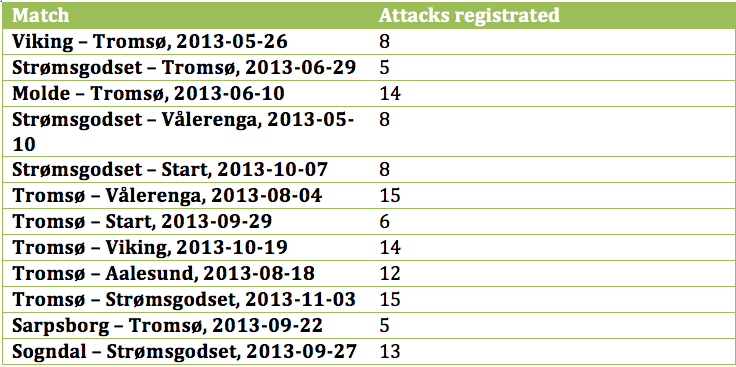
\includegraphics[width=1\textwidth]{images/evaluation/matched_regged.png}
\caption{Matches that have been captured and persisted into the database}
\label{fig:matches_regged}
\end{figure}

\subsection{SAT as a tool for opponent analytic}
% SAT gives you valuable information about opponents that the current systems you use today don’t provide

In this user servey the assessors where asked how SAT is as a complementary opponent analytic tool. In the requirement process we specified that the system should to be a complementing tool and not a direct replacement of the systems in use. The results shown in figure \ref{fig:user_servery1} shows that most of the assessors values the information the system provides. 

\begin{figure}[ht!]
\centering
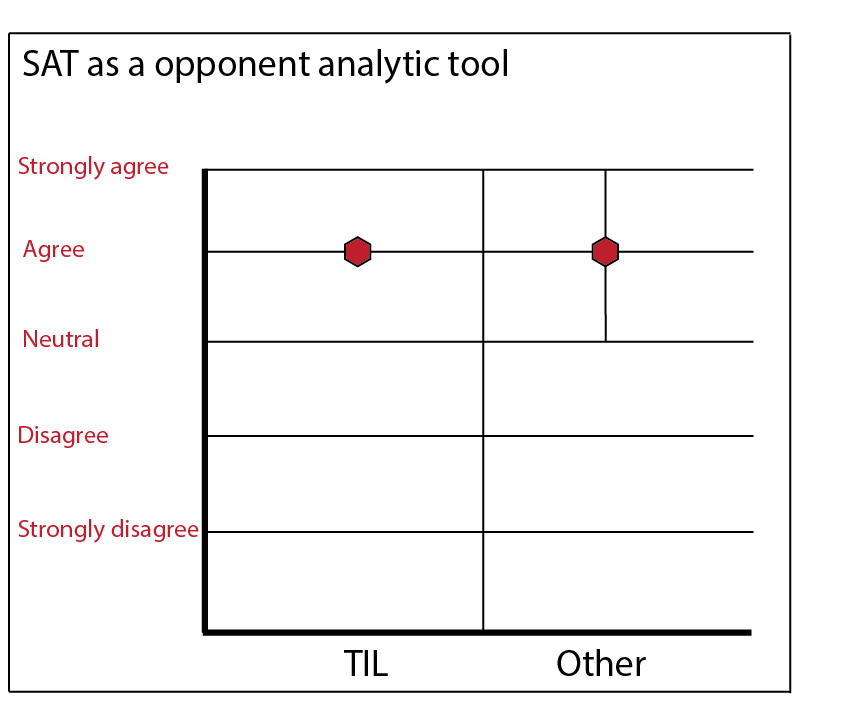
\includegraphics[width=1\textwidth]{images/evaluation/user_servery1}
\caption{User server 1}
\label{fig:user_servery1}
\end{figure}

Assessors not in the \ac{TIL} system do not necessarily use or have experience with an existing tool for opponent analytic. Therefor the statement was re-phrased. The assessors were asked how SAT is as an opponent analytic tool, a stand-alone product. The results listed at the right side in figure \ref{fig:user_servey1} shows that the majority of assessors was satisfied we the system with answers varying from neutral to strongly agree.

From these results we can conclude that the assessors view the Soccer Analytic Tool as a good system for providing information about soccer opponents. The information retrieved by using the tool is useful for analyzing your soccer opponent. The assessors would have the system rather not having it.

\subsection{SAT as a tool for identifying key players}

In this user servey the assessors where asked how SAT is as a tool for identifying key players in a soccer team. This was one of the main goals of the system. The results of the user servey is shown in figure \ref{fig:user_servery2}.

\begin{figure}[ht!]
\centering
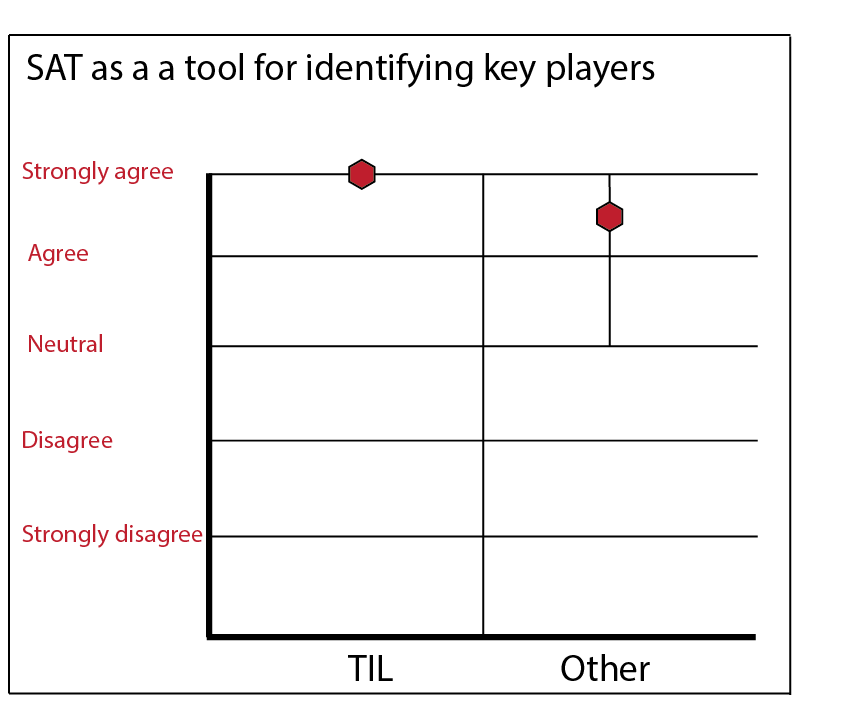
\includegraphics[width=1\textwidth]{images/evaluation/user_servery2}
\caption{User server 2}
\label{fig:user_servery2}
\end{figure}

We can see from the results of the user servey that the assessors agree that the system lets you identify key players in the opponent team. The varying from neutral to strongly agree.

\subsection{UI-performance}
UI performance was measured by testing the most content rich web page the team analytic page for \ac{TIL}. All the response times were measured by doing 20 samples. Tests where run at localhost with server and database running on the same machine, meaning that a further increase in time would likely be seen if the system was in production. Figure \ref{fig:uiperform} lists the results.

\begin{figure}[ht!]
\centering
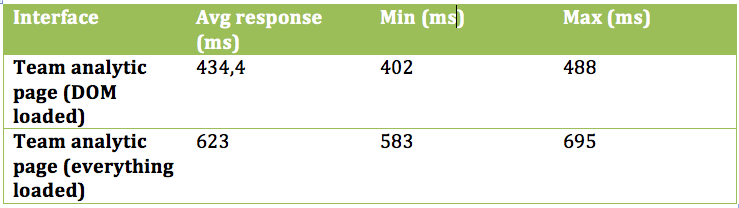
\includegraphics[width=1\textwidth]{images/evaluation/uipeform}
\caption{UI Performance test results. }
\label{fig:uiperform}
\end{figure}

Two tests were run to see the difference of a DOM load and a fully page load (all requests to the back-end done). The difference between the two is that in the latter we also add the time for the requests for team statistics as these requests are run when the JavaScript code is executed. 

The last test 

The results show that we are below the 1000ms threshold in both tests Nielsen \cite{nielsen} suggested. 

\subsection{Compatibility}

Figure \ref{fig:compa} shows the result after running the page in different web browsers with the PowerMapper tool. The results shows that the web page works in most browsers except from some issues in older Internet Explorer versions. We can conclude that the page has good compatibility with different web browsers making in accessible on many platforms.

\begin{figure}[ht!]
\centering
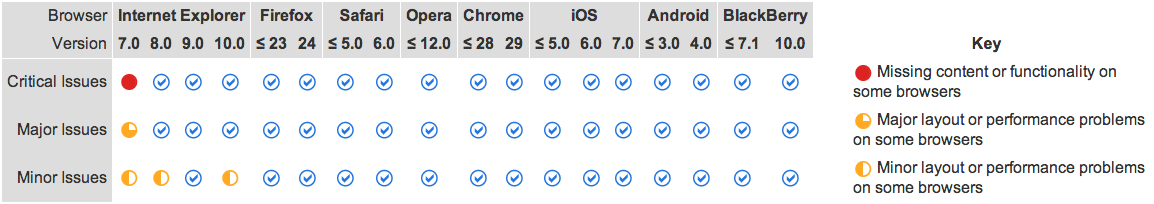
\includegraphics[width=1\textwidth]{images/evaluation/compa}
\caption{Compatibility test by running the web page in different browsers. Screenshot from powermapper.com free trial version}
\label{fig:compa}
\end{figure}

\section{Discussion}
\subsection{Input}

Perhaps the biggest limitation of the system is that it requires manual work to be functional. The system requires a lot of manually work to be operational as an opponent analytic tool. Up to one hour is the normal time spent capturing all data for a match with the current capture interface. On average, teams across the top four top leagues (La Liga, Premier League, Serie A and Bundesliga) took about 13 shots per match, measured in the 2010/11 season \cite{soccerbynumbers}. This means you will have possible have 26 attacks to capture for each match. 

In section \ref{sec:capprocess} it is mentioned that you have to store the players by their ID. IDs are only found in the database. Instead of this a player selector interface could have been developed letting you just click on an image of the player involved and the ID will be automatic inserted in. We suggest you can save up to 20 minutes by having this feature added.

\subsection{Accuracy}

There is minimal quality checking of the input data except from the match view page that lists every attack captured, meant for external operators to verify the data. Other than that you have to trust the operator that is capturing match data. The input is to some degree subjective for some data like identifying breakthroughs. In some cases one operator may say that it was a breakthrough and another operator does not agree. This may not be the biggest problem if you set some rules to follow for the operators. Identifying the zone for an event can also be a bit tricky. Especially, in soccer stadiums that have a low camera angel when being filmed. 

In our test data an average match is around 31.6kb size large, but we only capture attacks from one team. However, it is nothing in comparison with ZXY where a match is around 500-700mb. A more fear comparison would be against Opta’s data size for a match, as they are more in the same genre as our system, using only manual input. As previously mentioned, they capture every pass in the game meaning that they most likely store more data per match than our system. Another question is do you need this extra data to get a good opponent analytic system.

\subsection{Domain model}
The domain model has been dedicated a lot of time to in the process of defining and building the system. It was crucial to have a domain model that reflected what type of opponent analytic information the system should give the end-user. What is enough data? Having a larger domain model would increase time spent in the process of capturing data. 

A thing that could have been changed to get more precise analytic information is how breakthroughs are represented in the database. The current solutions store each type of breakthrough as text saying where on the pitch the breakthrough came from. Rather than this, we could have taken advantage of the already defined dividing of the pitch. This would have given use more precise data to present to the end-user.

\subsection{UI Performance}

A thing to take into consideration is the amount of matches in the database under the tests. A system in production would contain a lot more matches and would increase the response time. 

The team analytic page contains a lot of information. 

In a \ac{SPA} you don't necessary get all the files at once, but when you need them. On render, the web browser will first get the root \ac{HTML} document and then start requesting all other files that is referenced in the document, like \ac{CSS} and JavaScript files. Bundling all JavaScript files can to one file would save a lot of network traffic. Doing a reload of the team analytic page (non 303 Not Modified status codes) Google Developer Tools reports that total 55 requests is done to the back-end, fetching various files and requests to the REST API.

\subsection{Scalability}

Not in requirement

database size...

Write about scalability elasticsearch and node.js.

In the system it is clear that it is the storage that is the bottleneck of the system. It is the only component that does any computation. The client only gets data from the back-end and present it. The back-end 

\subsection{Usability}

End users did comment about graphical components on the client. Several assessors noted that improving the graphical components would increase the overall experience of the system and make the system easier to use. This has not been one of the main focuses during the development of the system. Drawing from the results of the user servers the system must be to some degree usable in the way of presenting analytic information to the user. Most of  different illustration techniques are used by combining HTML5 features and JavaScript library's to illustrate analytic information. 
Also the results of the user servey suggests that the




 
\acresetall

% Conclusion
\chapter{Conclusion} \label{Conclusion}
This chapter presents our achievements, gives some concluding remarks and outlines possible future work.

In this project, develops and evaluates a system for capturing, persisting and presenting information in the field of soccer opponent analysis. Particularly we have focused on identifying key players in the opponent team 

\textit{This thesis will develop a system complementing the Muithu and Bagadus systems. Focus will be on soccer opponent analytics, where a data repository need to be developed capturing important events relevant for this type of analytics. Specially we want to identify the key players in a team. A user interface component providing the core information about the opponent should also be developed.}

In the requirement specification we stated what we wanted from the system; a system that identifies key players in the offensive play of a soccer team. We also wanted to be able to see where on the field the key players contribute from.

To conclude we can say that we have achieved that to a certain degree looking at the result of the user servery. Assessors in the evaluation agrees that the system provides you with useful information about soccer opponents. 

\subsection{Concluding Remarks}

Building a system for soccer is complex task. There is many different terms in the field making it hard to make a vocabulary for your system. Soccer experts also values information differently and can figure out completely different things from the same statistic. 


\section{Future Work}

\subsection{Quality checking}

Simple quality checks of the data can be added on the back-end:

\begin{itemize}
\item \emph{Players}: In attacks with more than two passes is register. The attack start player should be the same as the sender of the first pass, or with no passes, the player finishing the attack. 
\item \emph{Player IDs}: Checking that IDs in passes matches a ID for the team in the attack.
\item \emph{Other}: 
\end{itemize}

Including to this, the single match page could have been updated with delete and edit buttons for attacks. This for operators to be able to correct or delete wrong data.

\subsection{New queries}

There is still a lot more queries than can be done on the data gathered. Examples includes listing what type of passes players play; cross, pass, longball. The same goes for type of finishes; shot miss, shot target or shot goal. This would need to be discussed with experts in the domain to quantify what can be useful. However, there is many possibilities. 

\subsection{Two team view}

Giving the end users the possibility to see statistics for two teams at the same time. The statistic for one team itself might not be so interesting if you don't have something to compare it to.  Graphical components in the system could have had a way to select a team to compare with.

Another feature would be a team vs team page where two teams are compared up to each other.


\acresetall

% References
\bibliographystyle{plain}
\bibliography{readlist}

\appendix


\end{document}